\documentclass[12pt]{article}
% for test commit
\usepackage[utf8]{inputenc}
\usepackage{newunicodechar}
\usepackage{EngReport}
\usepackage{listings}
\usepackage{cancel}
\usepackage{comment}
\usepackage{amssymb}
\usepackage{amsthm}
\usepackage{amsmath}
\usepackage{graphicx}
\usepackage{setspace}
\usepackage{geometry}
\usepackage{xcolor}  % Required for coloring in listings

\graphicspath{{Images/}}
\onehalfspacing
\geometry{letterpaper, portrait, includeheadfoot=true, hmargin=1in, vmargin=1in}

% Define custom colors
\definecolor{myblue}{RGB}{0, 128, 255}
\definecolor{mygreen}{RGB}{34, 139, 34}
\definecolor{myorange}{RGB}{255, 140, 0}
\definecolor{mygray}{RGB}{128, 128, 128}
\definecolor{mypurple}{RGB}{148, 0, 211}
\definecolor{myred}{RGB}{255, 69, 0}

% Configure listings for Python with custom styles
\lstset{
    language=Python,             % Set language to Python
    basicstyle=\ttfamily\small,  % Use a smaller monospace font
    keywordstyle=\color{myblue}\bfseries,  % Keywords in blue and bold
    commentstyle=\color{mygreen}\itshape,  % Comments in green and italic
    stringstyle=\color{myorange},          % Strings in orange
    numberstyle=\color{mygray},            % Line numbers in gray
    identifierstyle=\color{mypurple},      % Functions and variables in purple
    morekeywords={print, len, range},      % Define additional Python keywords
    showstringspaces=false,                % Do not show spaces in strings
    breaklines=true,                       % Enable line breaking
    numbers=left,                          % Add line numbers to the left
    numbersep=5pt,                         % Space between line numbers and code
    frame=single,                          % Add a box around the code
    rulecolor=\color{mygray},              % Frame color
    moredelim=[is][\color{myred}]{@@}{@@}, % Custom inline LaTeX coloring
}

\begin{document}
\renewcommand{\familydefault}{\rmdefault}

\begin{titlepage}
    \null % This is a TeX command that does nothing but is necessary for vfill to work correctly
    \vfill
    \begin{center}
        {\fontsize{40}{48}\selectfont \bfseries MAT232 - Lecture 13}
        \vspace{20pt} \\
        {\LARGE after partial derivatives?} \\
        \vspace{20pt}
        \textbf{AlexanderTheMango}
        \vspace{8pt}
        \\ Prepared for February 24, 2025
    \end{center}
    \vfill
\end{titlepage}

\pagestyle{fancy}
\fancyhf{}
\setlength{\headheight}{30pt}
\renewcommand{\headrulewidth}{0.4pt}
\renewcommand{\footrulewidth}{0.4pt}
\lhead{\large \textbf{CSC232 UTM} \\ \textbf{Lecture 1}}
\rhead{\large \textbf{Winter 2025} \\ \textbf{Lecture on Jan 2025}}
\rfoot{\textbf{Page \thepage}}
\lfoot{}
\pagebreak
\normalsize

\section*{Parametric Equations}
Recall the following from high school and first-year calculus:

\begin{table}[h!]
\centering
\begin{tabular}{|c|c|}
\hline
\textbf{Equation Type}     & \textbf{Example}             \\ \hline
Cartesian Equation         & $y = x^2$                   \\ \hline
Function in Cartesian Form & $y = f(x) = x^2$            \\ \hline
Parametric Equation        & $\begin{cases} 
x = t \\ 
y = t^2 
\end{cases}$ \\ \hline
\end{tabular}
\caption{Comparison of equation representations}
\label{tab:equation_comparison}
\end{table}

\begin{figure}[h!]
\centering
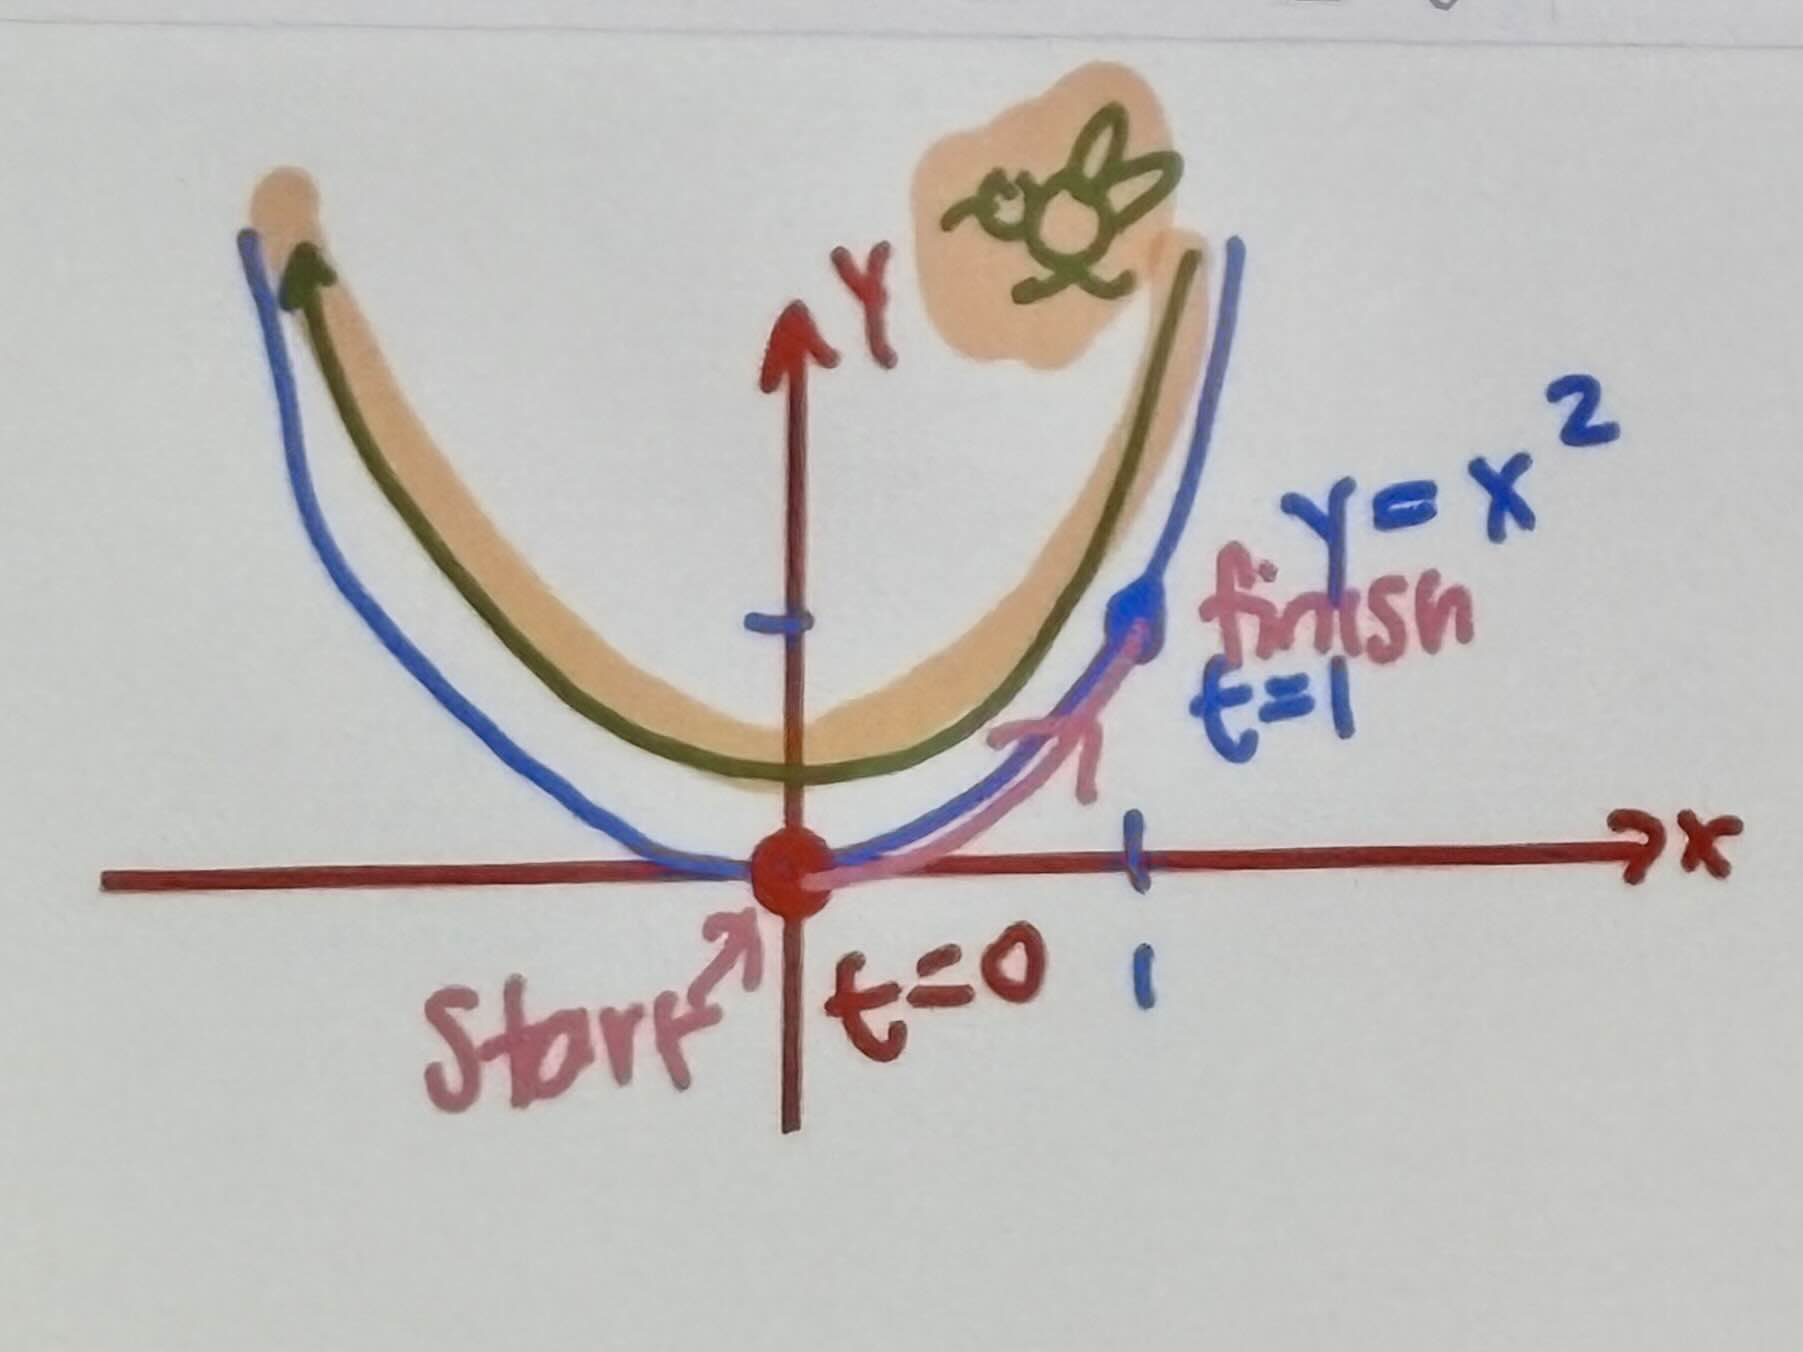
\includegraphics[width=0.6\textwidth]{parabola.jpg}
\caption{Graph of a parabola: $y = x^2$}
\label{fig:parabola}
\end{figure}

Parametric equations are of the form:
\[
x = f(t), \quad y = g(t), \quad t \in \mathbb{R}
\]

For example:
\[
x = t, \quad y = t^2, \quad t \in \mathbb{R}
\]
This yields points such as:
\[
(1, 1), \quad (0, 0), \quad (-1, 1)
\]

Alternatively:
\[
x = -t, \quad y = t^2, \quad t \in \mathbb{R}
\]
This yields points such as:
\[
(-1, 1), \quad (0, 0)
\]

\pagebreak

\section*{Drawing Parametric Equations}
Two methods are commonly used to sketch parametric equations:
\begin{itemize}
    \item Use a table of values for manual computation.
    \item Convert to a Cartesian equation (eliminate \( t \)) and sketch the graph, if possible.
\end{itemize}

Example:
Sketch \( x = t^2, y = t^3 \) for \( -\infty < t < \infty \).

Table of Values:
\[
\begin{array}{|c|c|c|c|}
\hline
t & x = t^2 & y = t^3 & (x, y) \\ \hline
2 & 4 & 8 & (4, 8) \\ \hline
1 & 1 & 1 & (1, 1) \\ \hline
0 & 0 & 0 & (0, 0) \\ \hline
-1 & 1 & -1 & (1, -1) \\ \hline
-2 & 4 & -8 & (4, -8) \\ \hline
\end{array}
\]

\begin{figure}[h!]
\centering
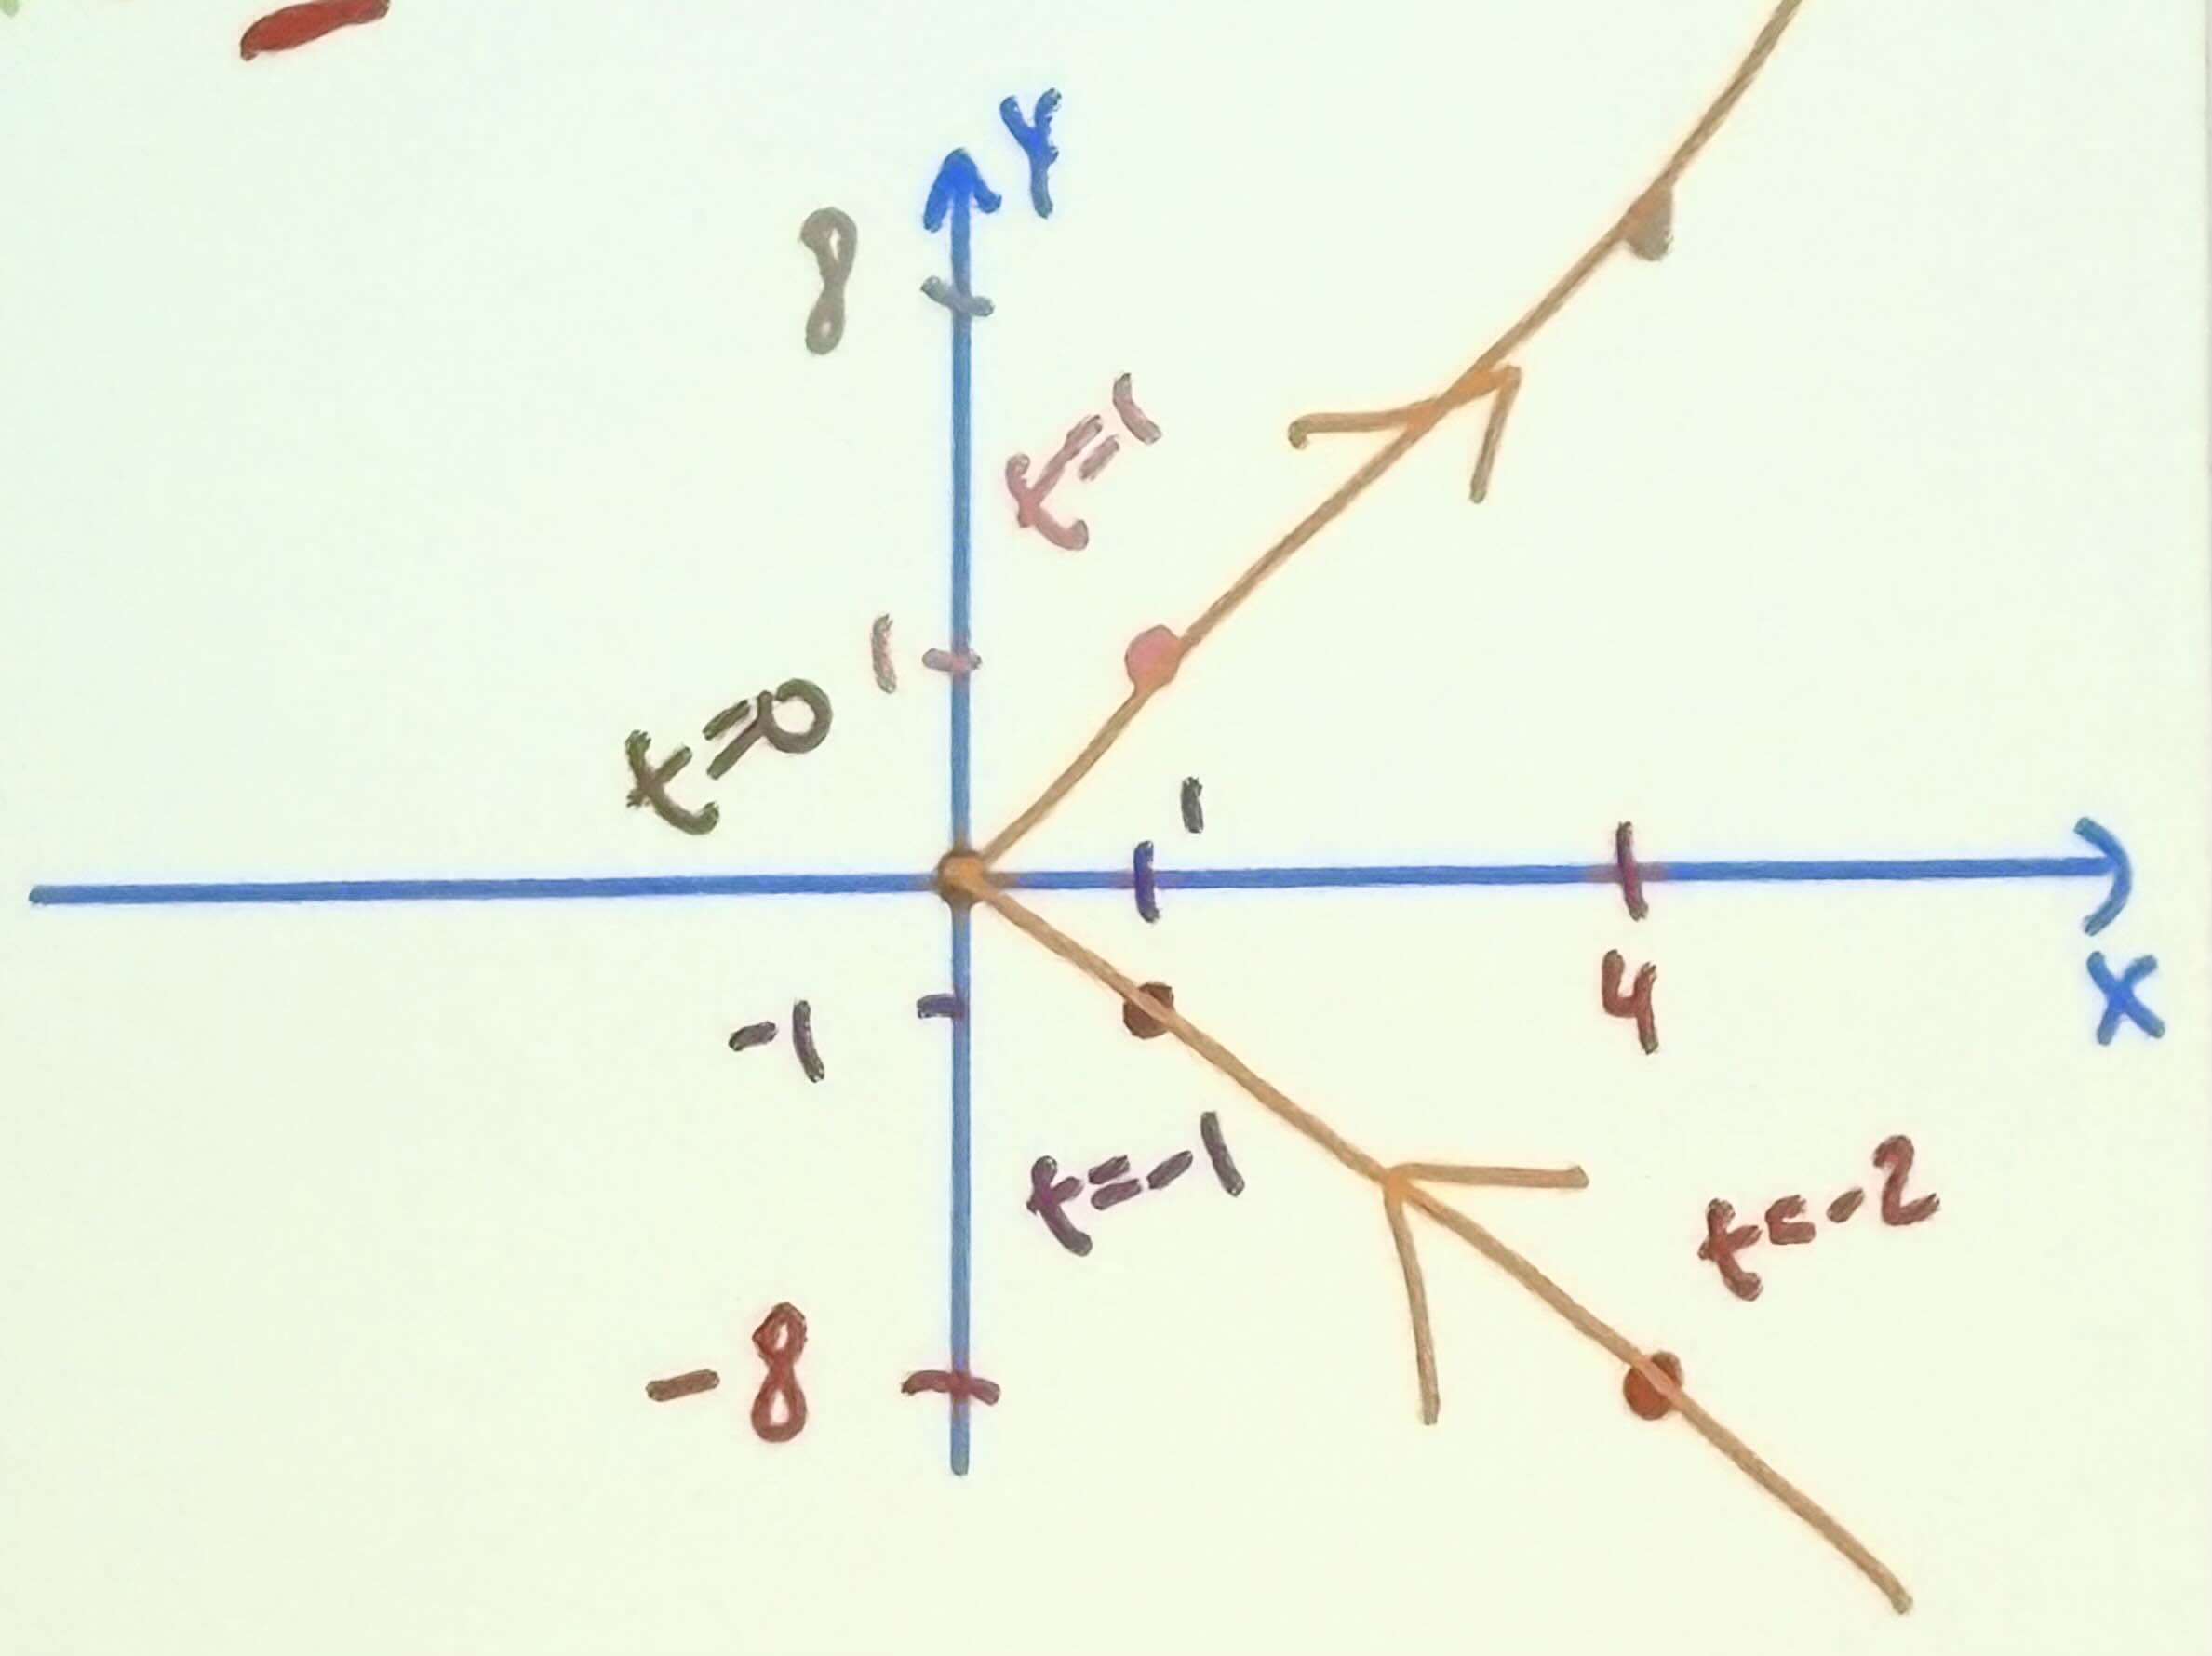
\includegraphics[width=0.6\textwidth]{sketching_example1.jpg}
\caption{Sketch of \( x = t^2, y = t^3 \)}
\label{fig:sketch_example1}
\end{figure}

\end{document}
